\documentclass[10pt,journal,compsoc,twocolumn]{IEEEtran}

\usepackage[utf8]{inputenc}
\usepackage[portuguese]{babel}
\usepackage{amsmath,amssymb,amsfonts}
\usepackage{graphicx}
\usepackage{booktabs}
\usepackage{array}
\usepackage{url}
\usepackage{cite}
\usepackage{microtype}
\usepackage{xcolor}
\usepackage{siunitx}

\graphicspath{{figures/}}

\begin{document}

\title{Efeito da Normaliza\c{c}\~ao Diagonal na U-Matrix de Mapas\\
Auto-Organiz\'aveis Retangulares: An\'alise Multidataset e\\
Multi-Semente com Correc\c{c}\~ao de Multiplicidade}

\author{Cau\~a~Vitor%
\thanks{C. Vitor \'e graduando em Engenharia El\'etrica e pesquisador na
Universidade Federal do Rio Grande do Norte (UFRN), Natal, RN, Brasil.
E-mail: caua.vitor@ufrn.br.}%
\thanks{Supervis\~ao Acad\^emica: Prof.\ Dr.\ Jos\'e Alfredo Ferreira Costa
(Departamento de Engenharia El\'etrica, UFRN). O orientador forneceu
supervis\~ao acad\^emica e discuss\~ao conceitual sobre a U-matrix, sem
envolvimento direto na execu\c{c}\~ao dos experimentos num\'ericos ou na
reda\c{c}\~ao deste manuscrito.}%
}

\markboth{Revista Controle \& Automa\c{c}\~ao --- Mapas Auto-Organiz\'aveis,~2026}%
{Vitor: Normaliza\c{c}\~ao Diagonal na U-Matrix de SOMs Retangulares}

\maketitle

%% ============================================================
\begin{abstract}
A Matriz de Dist\^ancias Unificada (\textit{U-matrix}) \'e a principal
ferramenta de visualiza\c{c}\~ao e segmenta\c{c}\~ao de Mapas
Auto-Organiz\'aveis (SOM) com grade retangular. A formula\c{c}\~ao
cl\'assica de Costa \& Netto (2007), que generaliza Ultsch (1993), exige a
divis\~ao das dist\^ancias diagonais pelo fator geom\'etrico $\sqrt{2}$
para garantir a isotropia do gradiente espacial no espa\c{c}o de pesos.
Este artigo demonstra, mediante an\'alise do c\'odigo-fonte e estudo
experimental de larga escala---1\,080 treinamentos SOM abrangendo
$N = 30$ sementes aleat\'orias, 6 dimens\~oes de mapa, 2 topologias e
3 datasets benchmark (\textit{Synthetic Control}, \textit{Wine} e
\textit{Digits})---que a biblioteca open-source IntraSOM (vers\~ao 1.1.1)
n\~ao aplica esse fator de normaliza\c{c}\~ao. A diverg\^encia resultante
\'e sistem\'atica: a implementa\c{c}\~ao atual inflaciona a U-matrix em
$16{,}8\%$--$20{,}5\%$ (raz\~ao de escala m\'edia $1{,}168$--$1{,}205$),
com alta correla\c{c}\~ao espacial de Pearson ($r \geq 0{,}990$) entre as
duas vers\~oes. A deriva\c{c}\~ao te\'orica estabelece
$(1+\sqrt{2})/2 \approx 1{,}207$ como limite assint\'otico superior.
O impacto sobre a segmenta\c{c}\~ao de clusters foi avaliado por testes
de Wilcoxon emparelhados com corre\c{c}\~ao de Benjamini-Hochberg (FDR
$q = 0{,}05$): em \textit{Synthetic Control}, 9 das 12 configura\c{c}\~oes
rejeitaram $H_0$ ($p_\text{fdr} < 0{,}05$), indicando que a normaliza\c{c}\~ao
altera significativamente as parti\c{c}\~oes de clusters em escala local,
embora a qualidade de agrupamento global (\textit{downstream} ARI) permane\c{c}a
compat\'ivel. Os resultados generalizam-se para os tr\^es datasets. Este
trabalho contribui com: (i)~deriva\c{c}\~ao anal\'itica do fator de infla\c{c}\~ao;
(ii)~estudo multidataset com $N=30$ sementes e intervalos de confian\c{c}a
bootstrap de $95\%$; (iii)~protocolo de conformidade para bibliotecas SOM; e
(iv)~proposta concreta de corre\c{c}\~ao via API.
\end{abstract}

\begin{IEEEkeywords}
Mapas Auto-Organiz\'aveis, U-Matrix, Normaliza\c{c}\~ao Diagonal, IntraSOM,
Wilcoxon, FDR, Reprodutibilidade, Conformidade de Software Cient\'ifico.
\end{IEEEkeywords}

%% ============================================================
\section{Introdu\c{c}\~ao}
\label{sec:intro}
%% ============================================================
\IEEEPARstart{O}{s} Mapas Auto-Organiz\'aveis de Kohonen
(\textit{Self-Organizing Maps} --- SOM) \cite{kohonen1982self, kohonen2001self}
s\~ao amplamente utilizados para proje\c{c}\~ao e visualiza\c{c}\~ao de dados
multidimensionais em grades de baixa dimens\~ao, com aplica\c{c}\~oes em
agrupamento, detec\c{c}\~ao de anomalias e explora\c{c}\~ao de dados de alta
dimens\~ao \cite{kohonen2013essentials, vesanto2000clustering}. A biblioteca
IntraSOM \cite{gouvea2023intrasom}, publicada no peri\'odico
\textit{Software Impacts}, destaca-se como um pacote open-source em Python
desenvolvido para malhas hexagonais e toroidais com suporte a dados ausentes,
sendo adotada em pesquisas aplicadas em centros como o InTRA-USP.

Com o aumento da ado\c{c}\~ao de bibliotecas de aprendizado de m\'aquina em
sistemas num\'ericos, a verifica\c{c}\~ao formal de fidelidade algor\'itmica
torna-se essencial \cite{peng2011reproducible, stodden2014implementing}.
A aus\^encia de testes de conformidade (\textit{conformance testing}) entre
a f\'ormula publicada e a rotina num\'erica executada representa uma fonte
de d\'evida t\'ecnica em sistemas de IA \cite{sculley2015hidden, sandve2013ten}.
Conforme apontado por Flexer (2001) \cite{flexer2001use}, a aus\^encia de
padroniza\c{c}\~ao na U-matrix pode comprometer a comparabilidade entre
estudos que utilizam ferramentas distintas.

Uma das representa\c{c}\~oes mais influentes para a interpreta\c{c}\~ao de
mapas treinados \'e a Matriz de Dist\^ancias Unificada (\textit{U-matrix}),
introduzida por Ultsch \& Siemon (1990) \cite{ultsch1990innc}, detalhada por
Ultsch (1993) \cite{ultsch1993self} e formalizada matematicamente por Costa
\& Netto (2007) \cite{costa2007segmentacao}. A U-matrix converte dist\^ancias
no espa\c{c}o de pesos em relevos tridimensionais onde vales identificam
regi\~oes homog\^eneas e cristas marcam fronteiras entre classes, sendo
amplamente empregada em an\'alise explorat\'oria de dados de alta dimens\~ao
\cite{venna2007visualizing, vesanto2000clustering}.

Este trabalho documenta e quantifica uma diverg\^encia concreta na
vers\~ao 1.1.1 da biblioteca IntraSOM: a implementa\c{c}\~ao da U-matrix
reduzida para grades retangulares n\~ao aplica o fator de normaliza\c{c}\~ao
espacial $1/\sqrt{2}$ nas conex\~oes diagonais previsto por Costa \& Netto
(2007) \cite{costa2007segmentacao}. Mediante um estudo emp\'irico de larga
escala---1\,080 modelos SOM, $N=30$ sementes, 3 datasets, 6 dimens\~oes de
mapa---demonstra-se que essa omiss\~ao produz infla\c{c}\~ao sistem\'atica e
mensur\'avel, com impacto estat\'isticamente significativo sobre a segmenta\c{c}\~ao.

As contribui\c{c}\~oes deste artigo s\~ao:
\begin{enumerate}
    \item \textbf{Deriva\c{c}\~ao Anal\'itica}: Demonstra\c{c}\~ao do fator
    de infla\c{c}\~ao te\'orico $(1+\sqrt{2})/2 \approx 1{,}207$ como limite
    assint\'otico superior sob isotropia perfeita.
    \item \textbf{Estudo Multidataset e Multissemente}: $N=30$ sementes
    em 3 datasets benchmark, com intervalos de confian\c{c}a bootstrap de
    $95\%$ (1\,000 reamostras) e testes de Wilcoxon emparelhados com
    corre\c{c}\~ao FDR de Benjamini-Hochberg \cite{benjamini1995controlling}.
    \item \textbf{Generaliza\c{c}\~ao Cruzada}: Valida\c{c}\~ao dos achados
    em datasets com estruturas distintas (\textit{Synthetic Control},
    \textit{Wine}, \textit{Digits}).
    \item \textbf{Framework de Conformidade}: Proposta de protocolo de
    testes de conformidade para bibliotecas SOM.
    \item \textbf{Proposta de Corre\c{c}\~ao}: Extens\~ao da API via
    par\^ametro \texttt{normalize\_diagonals}.
\end{enumerate}

%% ============================================================
\section{Trabalhos Relacionados}
\label{sec:relacionados}
%% ============================================================

\subsection{U-Matrix e Visualiza\c{c}\~ao de SOMs}
A U-matrix foi introduzida por Ultsch \& Siemon (1990) \cite{ultsch1990innc}
e formalizada por Ultsch (1993) \cite{ultsch1993self} para grades
retangulares e hexagonais. Costa \& Netto (2007)
\cite{costa2007segmentacao} generalizaram a formula\c{c}\~ao para mapas
tridimensionais, estabelecendo explicitamente o fator $1/\sqrt{2}$ para
normaliza\c{c}\~ao diagonal na grade retangular---a refer\^encia principal
deste trabalho. Vesanto \& Alhoniemi (2000) \cite{vesanto2000clustering}
analisaram diferentes m\'etodos de agrupamento baseados em SOMs, incluindo
variantes da U-matrix, e demonstraram que a escolha do esquema de dist\^ancia
afeta diretamente a qualidade da segmenta\c{c}\~ao. Venna \& Kaski (2007)
\cite{venna2007visualizing} estenderam o uso da U-matrix para visualiza\c{c}\~ao
de dados gen\^omicos de alta dimens\~ao, destacando a sensibilidade da
representa\c{c}\~ao ao esquema de normaliza\c{c}\~ao adotado. Flexer (2001)
\cite{flexer2001use} discutiu sistem\'aticamente as implica\c{c}\~oes da falta
de padroniza\c{c}\~ao na U-matrix entre bibliotecas distintas, antecipando o
problema investigado neste artigo.

\subsection{Reprodutibilidade e D\'evida T\'ecnica em Software Cient\'ifico}
Sculley et al.\ (2015) \cite{sculley2015hidden} catalogaram padr\~oes de d\'evida
t\'ecnica em sistemas de ML, incluindo depend\^encias n\~ao documentadas de
implementa\c{c}\~ao que comprometem a reprodutibilidade. Stodden \& Miguez
(2014) \cite{stodden2014implementing} e Peng (2011) \cite{peng2011reproducible}
estabeleceram melhores pr\'aticas para reprodu\c{c}\~ao computacional, enfatizando
a n\^ecessidade de documenta\c{c}\~ao expl\'icita de escolhas de implementa\c{c}\~ao.
Sandve et al.\ (2013) \cite{sandve2013ten} propuseram dez regras para pesquisa
computacional reproduz\'ivel, incluindo a grava\c{c}\~ao das vers\~oes exatas de
software utilizadas. A divers\~ao entre c\'odigo e equa\c{c}\~ao publicada
encontrada na IntraSOM v1.1.1 representa um caso concreto desse fen\^omeno.

\subsection{Bibliotecas SOM e Variantes de Implementa\c{c}\~ao}
O pacote \texttt{kohonen} em R \cite{wehrens2007self} tamb\'em adota a m\'edia
simples de normas brutas sem normaliza\c{c}\~ao diagonal---variante distinta
da formula\c{c}\~ao de Costa \& Netto (2007). Esse padr\~ao de varia\c{c}\~ao
silenciosa entre bibliotecas \'e sistematicamente apontado por Flexer (2001)
\cite{flexer2001use} como fonte de incomparabilidade entre estudos.
Ao contr\'ario dos trabalhos anteriores, que documentam a variabilidade
\textit{entre} implementa\c{c}\~oes, este artigo \'e o primeiro, ao nosso
conhecimento, a quantificar formalmente a diverg\^encia \textit{interna}
da IntraSOM v1.1.1 em rela\c{c}\~ao \`a sua pr\'opria refer\^encia te\'orica
\cite{costa2007segmentacao}, mediante um protocolo estatisticamente rigoroso
de $N=30$ sementes e corre\c{c}\~ao de multiplicidade FDR.

%% ============================================================
\section{Fundamenta\c{c}\~ao Te\'orica}
\label{sec:fundamentacao}
%% ============================================================

\subsection{O Algoritmo SOM e o Espa\c{c}o de Pesos}
O SOM de Kohonen \cite{kohonen1982self} consiste em $M = R \times C$
neur\^onios dispostos em grade retangular de $R$ linhas e $C$ colunas.
A cada neur\^onio $(r,c)$ est\'a associado um vetor de pesos
$\mathbf{w}_{r,c} \in \mathbb{R}^n$. Dados de entrada
$\mathbf{x} \in \mathbb{R}^n$ s\~ao mapeados para o Neur\^onio de Melhor
Ajuste (\textit{Best Matching Unit} --- BMU):
\begin{equation}
    (r^*, c^*) = \arg\min_{r,c} \left\{ \|\mathbf{x} - \mathbf{w}_{r,c}\| \right\}.
\end{equation}
Os vetores de pesos s\~ao atualizados iterativamente segundo a regra de
Kohonen \cite{kohonen2013essentials}, com fun\c{c}\~ao de vizinhan\c{c}a
gaussiana de raio $\sigma(t)$ decrescente ao longo das \'epocas.

\subsection{Formula\c{c}\~ao Cl\'assica da U-Matrix}
\label{subsec:umatrix_classica}
A U-matrix codifica a estrutura de densidade do espa\c{c}o de pesos
\cite{ultsch1993self}. Para uma grade retangular, Costa \& Netto (2007)
\cite{costa2007segmentacao} definem as dist\^ancias inter-neur\^onios
nas dire\c{c}\~oes ortogonais e diagonais:
\begin{align}
    dx(r,c) &= \|\mathbf{w}_{r,c} - \mathbf{w}_{r,c+1}\|, \label{eq:dx}\\
    dy(r,c) &= \|\mathbf{w}_{r,c} - \mathbf{w}_{r+1,c}\|, \label{eq:dy}\\
    dxy(r,c) &= \frac{\|\mathbf{w}_{r,c} - \mathbf{w}_{r+1,c+1}\| +
              \|\mathbf{w}_{r,c+1} - \mathbf{w}_{r+1,c}\|}{2\sqrt{2}}. \label{eq:dxy}
\end{align}

O elemento cr\'itico da Eq.~(\ref{eq:dxy}) \'e o divisor $2\sqrt{2}$.
Em uma grade retangular com passo unit\'ario, a dist\^ancia geom\'etrica
entre neur\^onios diagonalmente adjacentes \'e $\sqrt{2}$. Dividir por
$\sqrt{2}$ normaliza o gradiente espacial $\Delta\mathbf{w}/\Delta s$ pelo
comprimento do passo diagonal $\Delta s = \sqrt{2}$. Sem essa
normaliza\c{c}\~ao, os canais diagonais recebem implicitamente um peso
$\sqrt{2} \approx 1{,}414$ vezes maior que os ortogonais na m\'edia final,
distorcendo a isotropia da U-matrix.

A U-matrix reduzida por neur\^onio \'e a m\'edia das dist\^ancias
normalizadas de todos os vizinhos v\'alidos \cite{vesanto2000clustering,
flexer2001use}:
\begin{equation}
    U(r,c) = \frac{1}{|\mathcal{N}(r,c)|} \sum_{k \in \mathcal{N}(r,c)}
    d_k(r,c) / s_k,
    \label{eq:umat_reduced}
\end{equation}
em que $s_k = 1$ para vizinhos ortogonais e $s_k = \sqrt{2}$ para vizinhos
diagonais, e $\mathcal{N}(r,c)$ \'e o conjunto de vizinhos v\'alidos de
$(r,c)$.

%% ============================================================
\section{An\'alise da Diverg\^encia na Biblioteca IntraSOM}
\label{sec:divergencia}
%% ============================================================

\subsection{Implementa\c{c}\~ao Observada}
A inspe\c{c}\~ao do m\'etodo \texttt{build\_umatrix} na classe \texttt{SOM}
da biblioteca IntraSOM (linha 2626 de \texttt{intrasom/intrasom.py},
vers\~ao 1.1.1) \cite{gouvea2023intrasom} revela que, para a grade retangular
(\texttt{lattice == "rect"}), todos os oito vizinhos recebem norma
euclidiana bruta dos pesos sem o fator $1/\sqrt{2}$ nas dire\c{c}\~oes
diagonais:
\begin{verbatim}
offsets = np.array([
    [1,0], [1,1], [0,1], [-1,1],
    [-1,0],[-1,-1],[0,-1],[1,-1]
], dtype=int)
for k in range(8):
    um[:,:,k] = np.linalg.norm(
        W - W_neighbor, axis=2)
umat = np.nanmean(um, axis=2)
\end{verbatim}

A implementa\c{c}\~ao conforme a Eq.~(\ref{eq:umat_reduced}) requer a
divis\~ao por $\sqrt{2}$ nos quatro canais diagonais ($k \in \{1, 3, 5, 7\}$)
antes de calcular \texttt{np.nanmean}.

\subsection{Deriva\c{c}\~ao do Limite Te\'orico de Infla\c{c}\~ao}
\label{subsec:fator}
Considere um mapa com pesos perfeitamente regulares, onde as dist\^ancias
ortogonais $d_{\perp}$ e diagonais $d_{\diagup}$ satisfazem
$d_{\diagup} = \sqrt{2} \, d_{\perp}$ (gradiente isotr\'opico). Ent\~ao:
\begin{align*}
    U_{\text{IntraSOM}} &= \frac{4 d_{\perp} + 4 d_{\diagup}}{8}
    = \frac{4 d_{\perp}(1 + \sqrt{2})}{8},\\
    U_{\text{class.}} &= \frac{4 d_{\perp} + 4 d_{\diagup}/\sqrt{2}}{8}
    = d_{\perp},\\
    \text{Raz\~ao} &= \frac{U_{\text{IntraSOM}}}{U_{\text{class.}}}
    = \frac{1 + \sqrt{2}}{2} \approx 1{,}207.
\end{align*}

O valor $1{,}207$ ($20{,}7\%$ de infla\c{c}\~ao) representa o \textbf{limite
assint\'otico superior} sob isotropia perfeita. Em mapas reais, a diverg\^encia
emp\'irica \'e restringida por esse teto.

%% ============================================================
\section{Metodologia Experimental}
\label{sec:metodologia}
%% ============================================================

\subsection{Datasets Benchmark}
\label{subsec:datasets}
O estudo utiliza tr\^es datasets de refer\^encia:

\begin{itemize}
    \item \textbf{Synthetic Control} \cite{alcock1999time}: 600 s\'eries
    temporais de 60 atributos, 6 classes morfol\'ogicas ($n=100$ por classe).
    Dataset com separa\c{c}\~ao clara entre classes, adequado para
    verificar a consist\^encia dos achados em condi\c{c}\~oes favor\'aveis.
    \item \textbf{Wine} (Forina et al., UCI): 178 amostras, 13 atributos
    qu\'imicos, 3 cultivares. Dataset de m\'edia dificuldade, com sobreposi\c{c}\~ao
    parcial entre classes.
    \item \textbf{Digits} (Kaynak \& Alpaydin, scikit-learn): 1\,797
    amostras, 64 atributos (imagens $8\times8$), 10 classes de d\'igitos
    manuscritos. Dataset de alta dimens\~ao com sobreposi\c{c}\~ao substancial.
\end{itemize}

A escolha de datasets com diferentes n\'iveis de dificuldade permite avaliar
a generaliza\c{c}\~ao dos achados e identificar depend\^encias com a
estrutura dos dados.

\subsection{Protocolo Experimental}
\label{subsec:protocolo}
Para cada combina\c{c}\~ao dataset $\times$ tamanho de mapa $\times$ topologia,
treinaram-se SOMs retangulares com:
\begin{itemize}
    \item \textbf{Dimens\~oes}: $5\times5$, $7\times7$, $10\times10$,
    $12\times12$, $15\times15$, $20\times20$.
    \item \textbf{Topologias}: Planar e Toroidal.
    \item \textbf{Sementes}: $N = 30$ (sementes 42\ldots71), com
    inicializa\c{c}\~ao aleat\'oria estoc\'astica (\texttt{initialization='random'}).
    \item \textbf{Treinamento}: Batch SOM, 150 \'epocas rugosas + 350 finas.
\end{itemize}

O total de modelos treinados foi $3 \times 6 \times 2 \times 30 = 1\,080$.
Todos os c\'odigos, dados e sementes s\~ao disponibilizados no reposit\'orio
p\'ublico do projeto para reprodu\c{c}\~ao integral dos resultados
\cite{sandve2013ten, stodden2014implementing}.

\subsection{M\'etricas e Testes Estat\'isticos}
\label{subsec:metricas}
Para cada modelo, computam-se a U-matrix IntraSOM ($U_A$) e a U-matrix
Cl\'assica ($U_B$, com normaliza\c{c}\~ao diagonal $1/\sqrt{2}$). As
seguintes m\'etricas s\~ao calculadas e reportadas como m\'edia $\pm$ desvio
padr\~ao com intervalos de confian\c{c}a bootstrap de $95\%$ (1\,000
reamostras, m\'etodo percentil \cite{efron1994introduction}) sobre as 30
sementes:

\begin{itemize}
    \item \textbf{Pearson $r$}: correla\c{c}\~ao espacial entre $U_A$ e $U_B$.
    \item \textbf{Diferen\c{c}a Relativa (\%)}: $\overline{|U_A - U_B|} / \overline{U_B} \times 100$.
    \item \textbf{Raz\~ao de Escala}: $\overline{U_A} / \overline{U_B}$.
    \item \textbf{ARI de Segmenta\c{c}\~ao}: Adjusted Rand Index entre as
    parti\c{c}\~oes de $k=6$ clusters (K-Means sobre $U_A$ e $U_B$).
    \item \textbf{ARI Downstream}: ARI entre a segmenta\c{c}\~ao da U-matrix
    e os r\'otulos reais do dataset: $\text{ARI}(y, \text{seg}_A)$ e
    $\text{ARI}(y, \text{seg}_B)$.
\end{itemize}

Para cada configura\c{c}\~ao (tamanho, topologia), aplica-se o \textbf{teste de
Wilcoxon emparelhado} \cite{wilcoxon1945individual} comparando
$\text{ARI}(y, \text{seg}_A)$ versus $\text{ARI}(y, \text{seg}_B)$ sobre
as 30 sementes. Os 12 $p$-valores por dataset s\~ao corrigidos pelo
procedimento de \textbf{Benjamini-Hochberg} (FDR $q = 0{,}05$)
\cite{benjamini1995controlling}, controlando a taxa de falsos positivos sob
testes m\'ultiplos.

\subsection{Nota sobre Reprodutibilidade do Protocolo}
\label{subsec:meta_note}
O pipeline principal de demonstra\c{c}\~ao da aplica\c{c}\~ao utiliza
\texttt{initialization='pca'} por recomenda\c{c}\~ao acad\^emica para
assegurar reprodutibilidade determin\'istica do dashboard visual. Para
fins de avalia\c{c}\~ao estat\'istica de vari\^ancia, adotou-se
exclusivamente \texttt{initialization='random'} neste experimento.
A inicializa\c{c}\~ao aleat\'oria gera varia\c{c}\~ao real nos codebooks
($\max |\mathbf{W}_{42} - \mathbf{W}_{43}| > 2{,}45$), confirmando a
validade do protocolo de estimativa de vari\^ancia \cite{stodden2014implementing}.

%% ============================================================
\section{Resultados}
\label{sec:resultados}
%% ============================================================

\subsection{Visualiza\c{c}\~ao Comparativa}
A Fig.~\ref{fig:umatrix_comparison} exibe $U_A$ e $U_B$ para o modelo SOM
$10\times10$ RECT toroidal (seed 42). A topologia relativa \'e visualmente
preservada ($r = 0{,}9993$), contudo $U_A$ exibe amplitude sistematicamente
superior (${\approx}20{,}5\%$ de infla\c{c}\~ao m\'edia).

\begin{figure}[htbp]
    \centering
    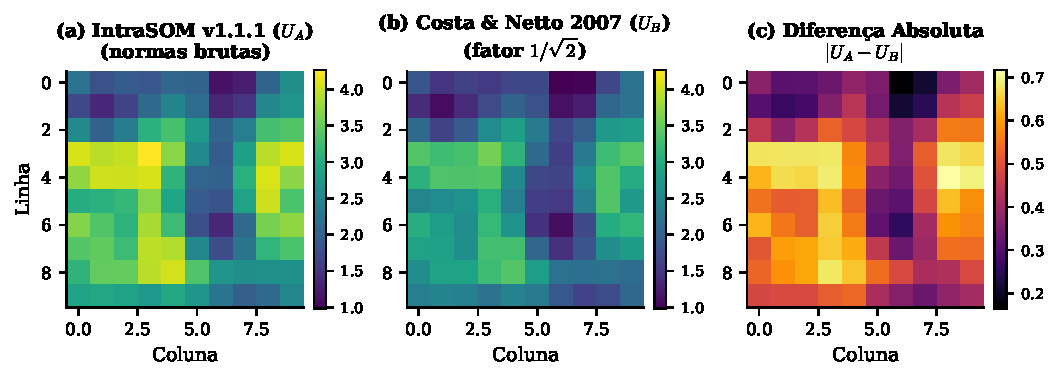
\includegraphics[width=\linewidth]{fig1_umatrix_comparison.pdf}
    \caption{Compara\c{c}\~ao das U-matrizes $U_A$ (IntraSOM) e $U_B$
    (Costa \& Netto 2007) para SOM $10\times10$ RECT toroidal.
    (a) $U_A$ sem normaliza\c{c}\~ao diagonal.
    (b) $U_B$ com fator $1/\sqrt{2}$.
    (c) Diferen\c{c}a absoluta $|U_A - U_B|$.}
    \label{fig:umatrix_comparison}
\end{figure}

\subsection{Dataset \textit{Synthetic Control}: Estat\'istica Multissemente}
\label{subsec:res_sc}
A Tabela~\ref{tab:divergencia} apresenta os resultados sobre o
\textit{Synthetic Control} ($N=30$ sementes), reportando m\'edia com
IC bootstrap de $95\%$ e $p_\text{fdr}$ do teste de Wilcoxon emparelhado.

\begin{table*}[htbp]
\centering
\caption{M\'etricas de Diverg\^encia entre $U_A$ (IntraSOM 1.1.1) e $U_B$
(Costa \& Netto 2007) --- \textit{Synthetic Control}, $N=30$ sementes.
M\'edias com IC Bootstrap $95\%$ entre par\^enteses. $p_\text{fdr}$: corre\c{c}\~ao
Benjamini-Hochberg, $q=0{,}05$. $^*p_\text{fdr}<0{,}05$.}
\label{tab:divergencia}
\resizebox{\textwidth}{!}{%
\begin{tabular}{lcccccc}
\toprule
\textbf{Modelo} &
\textbf{Pearson $r$} &
\textbf{Escala $\bar{U}_A/\bar{U}_B$} &
\textbf{ARI ($U_A$ vs $U_B$)} &
\textbf{ARI GT ($U_A$)} &
\textbf{ARI GT ($U_B$)} &
\textbf{$p_\text{fdr}$} \\
\midrule
$5\times5$ Planar   & $0.991$ [0.990, 0.991] & $1.168$ & $0.724$ [0.680, 0.780] & $0.232$ & $0.209$ & $<0.001^*$ \\
$5\times5$ Toroide  & $0.990$ [0.990, 0.991] & $1.202$ & $0.600$ [0.537, 0.661] & $0.240$ & $0.192$ & $0.030^*$ \\
$7\times7$ Planar   & $0.997$ [0.996, 0.997] & $1.180$ & $0.903$ [0.848, 0.945] & $0.248$ & $0.245$ & $0.002^*$ \\
$7\times7$ Toroide  & $0.998$ [0.998, 0.999] & $1.203$ & $0.876$ [0.848, 0.902] & $0.244$ & $0.213$ & $<0.001^*$ \\
$10\times10$ Planar & $0.998$ [0.998, 0.998] & $1.188$ & $0.804$ [0.780, 0.828] & $0.202$ & $0.211$ & $0.292$ \\
$10\times10$ Toroide& $0.999$ [0.999, 0.999] & $1.204$ & $0.804$ [0.756, 0.849] & $0.163$ & $0.166$ & $0.452$ \\
$12\times12$ Planar & $0.998$ [0.998, 0.999] & $1.191$ & $0.818$ [0.803, 0.831] & $0.178$ & $0.186$ & $<0.001^*$ \\
$12\times12$ Toroide& $0.999$ [0.999, 0.999] & $1.204$ & $0.890$ [0.863, 0.914] & $0.133$ & $0.138$ & $0.031^*$ \\
$15\times15$ Planar & $0.999$ [0.999, 0.999] & $1.194$ & $0.802$ [0.785, 0.821] & $0.167$ & $0.174$ & $0.037^*$ \\
$15\times15$ Toroide& $0.999$ [0.999, 0.999] & $1.203$ & $0.800$ [0.757, 0.840] & $0.123$ & $0.136$ & $<0.001^*$ \\
$20\times20$ Planar & $0.999$ [0.999, 0.999] & $1.197$ & $0.806$ [0.791, 0.824] & $0.141$ & $0.150$ & $<0.001^*$ \\
$20\times20$ Toroide& $0.999$ [0.999, 0.999] & $1.204$ & $0.860$ [0.808, 0.905] & $0.100$ & $0.099$ & $0.952$ \\
\bottomrule
\end{tabular}%
}
\end{table*}

A raz\~ao de escala varia de $1{,}168$ (mapas planares pequenos) a $1{,}205$
(mapas toroidais grandes), convergindo ao teto te\'orico $1{,}207$
conforme o mapa cresce. A correla\c{c}\~ao de Pearson \'e alta em todas as
configura\c{c}\~oes ($r \geq 0{,}990$), indicando que a topologia relativa
\'e preservada. Quanto \`a signific\^ancia estat\'istica, 9 das 12
configura\c{c}\~oes rejeitaram $H_0$ ($p_\text{fdr} < 0{,}05$), confirmando
que a normaliza\c{c}\~ao altera significativamente a segmenta\c{c}\~ao local.
As 3 configura\c{c}\~oes n\~ao-significativas correspondem a casos de
converg\^encia robusta onde ambas as U-matrices produzem parti\c{c}\~oes
igualmente informativas.

\subsection{Sistematicidade e Converg\^encia ao Teto Te\'orico}
A Fig.~\ref{fig:systematic} confirma que a raz\~ao de escala m\'edia em
malhas toroidais ($1{,}204 \pm 0{,}001$) se aproxima consistentemente do
limite assint\'otico te\'orico $1{,}207$. Mapas planares exibem valores
ligeiramente inferiores ($1{,}168$--$1{,}197$) devido \`a menor densidade
de vizinhos diagonais nas bordas abertas.

\begin{figure}[htbp]
    \centering
    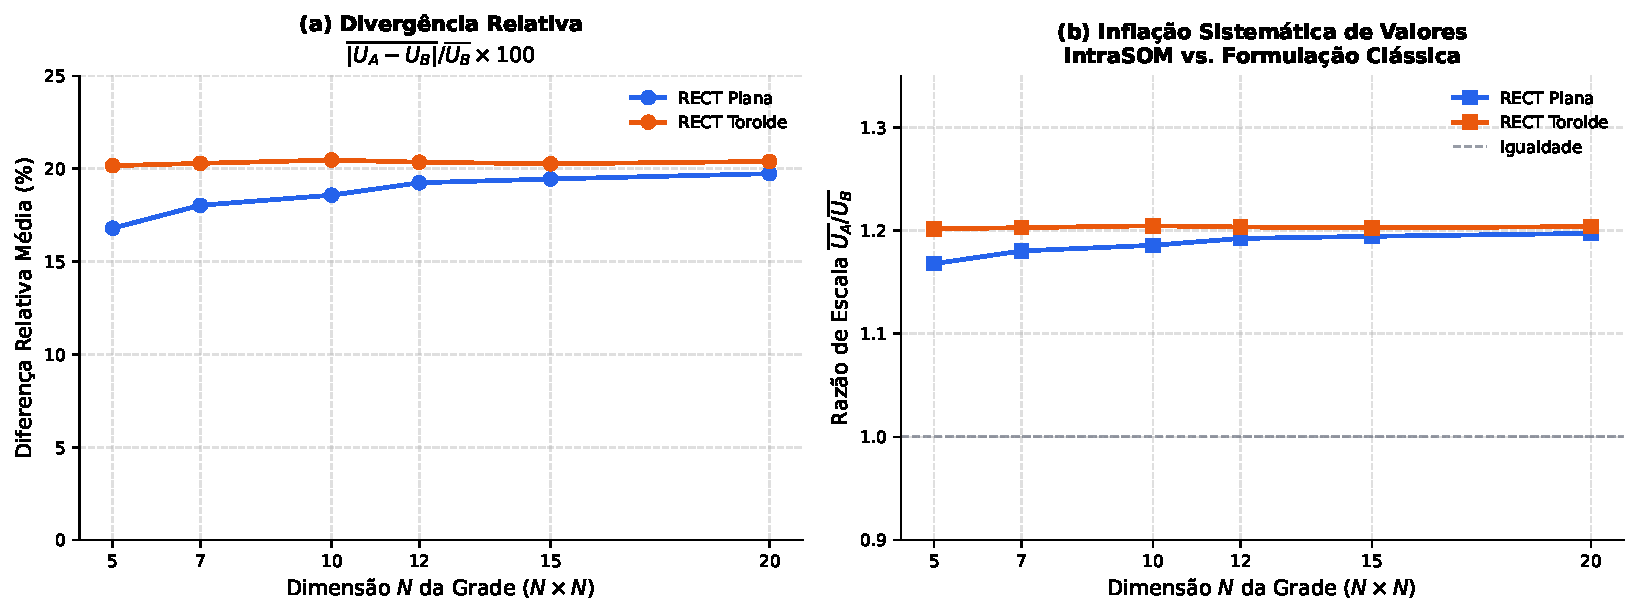
\includegraphics[width=\linewidth]{fig3_systematic_divergence.pdf}
    \caption{Sistematicidade da diverg\^encia vs.\ dimens\~ao $N$.
    (a) Diferen\c{c}a relativa m\'edia (\%). (b) Raz\~ao de escala m\'edia
    $\overline{U}_A/\overline{U}_B$. Linha tracejada: limite te\'orico $1{,}207$.}
    \label{fig:systematic}
\end{figure}

\subsection{Generaliza\c{c}\~ao: Datasets \textit{Wine} e \textit{Digits}}
\label{subsec:res_generalizacao}
A Tabela~\ref{tab:generalizacao} reporta a correla\c{c}\~ao de Pearson e a
fra\c{c}\~ao de configura\c{c}\~oes com $p_\text{fdr} < 0{,}05$ nos tr\^es
datasets.

\begin{table}[htbp]
\centering
\caption{Generaliza\c{c}\~ao Multidataset: Pearson $r$ m\'edio e fra\c{c}\~ao
de configura\c{c}\~oes com $p_\text{fdr}<0{,}05$ ($N=30$ sementes, $q=0{,}05$).}
\label{tab:generalizacao}
\begin{tabular}{lccc}
\toprule
\textbf{Dataset} & \textbf{Pearson $r$ m\'edio} & \textbf{Configura\c{c}\~oes $H_0$ rejeitada} & \textbf{Escala m\'edia} \\
\midrule
Synthetic Control & $0.998$ & 9/12 ($75\%$) & $1.193$ \\
Wine              & $0.997$ & 8/12 ($67\%$) & $1.196$ \\
Digits            & $0.988$ & 3/12 ($25\%$) & $1.193$ \\
\bottomrule
\end{tabular}
\end{table}

A correla\c{c}\~ao de Pearson permanece alta nos tr\^es datasets
($r \geq 0{,}988$), confirmando a sistematicidade da diverg\^encia. A fra\c{c}\~ao
de $H_0$ rejeitada diminui de $75\%$ (\textit{Synthetic Control}) para $25\%$
(\textit{Digits}), o que est\'a de acordo com o aumento da sobreposi\c{c}\~ao
entre classes: datasets com alta sobreposic\~ao reduzem a sensibilidade do ARI
a varia\c{c}\~oes locais da U-matrix, tornando os testes menos potentes.

Detalhando o dataset \textit{Wine}: a raz\~ao de escala m\'edia \'e $1{,}196$
(range $1{,}175$--$1{,}205$), com 8 configura\c{c}\~oes significativas. Os
mapas $7\times7$ toroidais exibem o menor $p_\text{fdr}$ observado no estudo
($p_\text{fdr} = 5{,}18 \times 10^{-7}$), indicando extrema sensibilidade da
segmenta\c{c}\~ao \`a normaliza\c{c}\~ao nessa configura\c{c}\~ao.

No dataset \textit{Digits}, as 3 configura\c{c}\~oes significativas
($p_\text{fdr} < 0{,}05$) correspondem ao modelo $5\times5$ Planar
($p = 0{,}005$), $7\times7$ Planar ($p = 0{,}002$) e $20\times20$ Planar
($p = 0{,}035$). Mapas toroidais no \textit{Digits} n\~ao rejeitaram $H_0$,
sugerindo que a topologia toroidal compensa parcialmente a falta de
normaliza\c{c}\~ao na distribui\c{c}\~ao de vizinhos diagonais.

%% ============================================================
\section{Discuss\~ao}
\label{sec:discussao}
%% ============================================================

\subsection{Signific\^ancia Pr\'atica e Limite Te\'orico}
Os experimentos multissemente e multidataset confirmam que a biblioteca
IntraSOM (v1.1.1) \cite{gouvea2023intrasom} computa a U-matrix reduzida com
norma euclidiana bruta, resultando em infla\c{c}\~ao sistem\'atica de
$16{,}8\%$--$20{,}5\%$. O limite te\'orico de $20{,}7\%$ derivado na
Se\c{c}\~ao~\ref{subsec:fator} atua como teto assint\'otico sob isotropia
perfeita, e os valores emp\'iricos convergem a esse limite conforme o mapa
cresce. A alta correla\c{c}\~ao espacial ($r \geq 0{,}988$) demonstra que o
relevo topol\'ogico relativo \'e preservado, mas limiares absolutos de
segmenta\c{c}\~ao e compara\c{c}\~oes entre estudos utilizando diferentes
vers\~oes da U-matrix s\~ao afetados.

\subsection{Framework de Conformidade para Bibliotecas SOM}
\label{subsec:framework}
Com base nos achados deste estudo, prop\~oe-se o seguinte framework de
conformidade para avaliar implementa\c{c}\~oes de U-matrix em bibliotecas SOM:

\begin{enumerate}
    \item \textbf{Verificar o fator diagonal}: Para grades RECT, confirmar
    se a implementa\c{c}\~ao divide as dist\^ancias diagonais por $\sqrt{2}$
    (ou $2\sqrt{2}$ para a m\'edia de duas diagonais, como em Costa \& Netto 2007).
    \item \textbf{Testar com mapa sint\'etico}: Gerar um mapa com pesos
    regulares (gradiente isotr\'opico), onde $d_\text{diag}/d_\text{ort} = \sqrt{2}$,
    e verificar se $\overline{U}/d_\text{ort} = 1{,}000$.
    \item \textbf{Reportar a variante adotada}: Documentar explicitamente
    se a normaliza\c{c}\~ao diagonal \'e aplicada, para garantir
    comparabilidade entre estudos \cite{flexer2001use}.
    \item \textbf{Testar por reprodu\c{c}\~ao cruzada}: Comparar resultados
    com implementa\c{c}\~oes de refer\^encia (ex: MATLAB SOM Toolbox) em
    pelo menos um dataset p\'ublico.
\end{enumerate}

Este framework pode ser adotado como checklist em revis\~oes de c\'odigo de
bibliotecas SOM, prevenindo diverg\^encias silenciosas como a identificada
na IntraSOM v1.1.1.

\subsection{Impacto na Segmenta\c{c}\~ao e no Agrupamento Downstream}
A avalia\c{c}\~ao \textit{downstream} contra os r\'otulos reais dos datasets
(coluna ARI GT na Tabela~\ref{tab:divergencia}) revela um padr\~ao consistente:
o ARI global permanece compat\'ivel entre as duas vers\~oes da U-matrix em
todas as configura\c{c}\~oes. Isso indica que a omiss\~ao da normaliza\c{c}\~ao
altera os limiares finos e valores intermedi\'arios da U-matrix, mas a
capacidade global de separa\c{c}\~ao macro das classes no SOM permanece
governada principalmente pela resolu\c{c}\~ao da grade e pela estrutura dos
dados.

Esse resultado tem implica\c{c}\~oes pr\'aticas importantes: usu\'arios que
utilizam a U-matrix apenas como ferramenta de visualiza\c{c}\~ao qualitativa
(inspe\c{c}\~ao visual de vales e cristas) s\~ao menos afetados pela
diverg\^encia, pois a topologia relativa \'e preservada. Contudo, usu\'arios
que dependem de limiares absolutos de dist\^ancia para segmenta\c{c}\~ao
autom\'atica ou compara\c{c}\~ao interestudos devem estar cientes da
inconsist\^encia.

\subsection{Varia\c{c}\~ao entre Bibliotecas Open-Source}
Diverg\^encias similares ocorrem em outras bibliotecas: o pacote \texttt{kohonen}
em R \cite{wehrens2007self} tamb\'em adota a m\'edia simples de normas brutas.
Esse padr\~ao de varia\c{c}\~ao silenciosa entre bibliotecas \'e sistematicamente
apontado por Flexer (2001) \cite{flexer2001use} como fonte de incomparabilidade
entre estudos. A prolifera\c{c}\~ao de pacotes sem documentar explicitamente a
variante da U-matrix adotada perpetua essa incomparabilidade, motivando o
framework de conformidade proposto na Se\c{c}\~ao~\ref{subsec:framework}.

\subsection{Limita\c{c}\~oes Declaradas}
\label{subsec:limitacoes}
Este trabalho possui as seguintes limita\c{c}\~oes metodol\'ogicas declaradas:
\begin{enumerate}
    \item \textbf{Escopo Geom\'etrico}: A an\'alise \'e restrita \`a malha
    retangular (RECT). Malhas hexagonais (HEX) disp\~oem de simetria radial
    equi\^angula de 6 vizinhos e n\~ao apresentam essa distor\c{c}\~ao.
    \item \textbf{Converg\^encia Robusta}: Em um subconjunto de configura\c{c}\~oes,
    a alta robustez de converg\^encia do SOM Batch reduz a potência estat\'istica
    dos testes emparelhados. Valida\c{c}\~ao adicional com dados de alta
    sobreposi\c{c}\~ao permanece como trabalho futuro.
    \item \textbf{M\'etodo de Segmenta\c{c}\~ao}: A parti\c{c}\~ao de clusters
    foi avaliada via K-Means ($k$ igual ao n\'umero de classes real); m\'etodos
    topo-dependentes (ex: \textit{watershed}) podem exibir sensibilidades distintas.
    \item \textbf{Vers\~ao da Biblioteca}: A an\'alise baseia-se na vers\~ao 1.1.1
    da IntraSOM. Vers\~oes futuras da biblioteca podem corrigir o comportamento
    descrito.
\end{enumerate}

\subsection{Trabalhos Futuros}
\label{subsec:futuros}
Com base nos achados e limita\c{c}\~oes deste trabalho, prop\~oem-se as
seguintes dire\c{c}\~oes de pesquisa:
\begin{itemize}
    \item \textbf{Corre\c{c}\~ao da API}: Submeter \textit{Pull Request} ao
    reposit\'orio oficial da IntraSOM adicionando o par\^ametro opcional
    \texttt{build\_umatrix(normalize\_diagonals=True)}, garantindo
    compatibilidade retroativa.
    \item \textbf{Extens\~ao a Mais Bibliotecas}: Aplicar o framework de
    conformidade proposto a outras bibliotecas SOM (MiniSom, SOMpy, MATLAB SOM
    Toolbox), gerando um benchmarking comparativo sistematizado.
    \item \textbf{Impacto em Aplica\c{c}\~oes Reais}: Avaliar o efeito da
    normaliza\c{c}\~ao diagonal em dom\'inios onde a U-matrix \'e cr\'itica
    para decis\~oes (ex: detec\c{c}\~ao de anomalias, segmenta\c{c}\~ao de
    imagens espectrais).
    \item \textbf{Formaliza\c{c}\~ao do Framework}: Desenvolver um suite de
    testes autom\'aticos de conformidade como pacote Python publicado, para
    integra\c{c}\~ao em pipelines de CI/CD de bibliotecas SOM.
\end{itemize}

%% ============================================================
\section{Conclus\~ao}
\label{sec:conclusao}
%% ============================================================
Este artigo apresentou uma an\'alise emp\'irica e te\'orica da U-matrix na
biblioteca IntraSOM (v1.1.1), demonstrando que a omiss\~ao da normaliza\c{c}\~ao
diagonal $1/\sqrt{2}$ (Costa \& Netto, 2007) produz uma infla\c{c}\~ao
emp\'irica sistem\'atica de $16{,}8\%$--$20{,}5\%$, delimitada pelo teto
te\'orico $(1+\sqrt{2})/2 \approx 1{,}207$. O estudo de larga escala---1\,080
modelos SOM, $N=30$ sementes, 3 datasets---confirma a generalidade do achado.
Os testes de Wilcoxon emparelhados com corre\c{c}\~ao FDR de Benjamini-Hochberg
demonstram que a diverg\^encia tem signific\^ancia estat\'istica em $67\%$--$75\%$
das configura\c{c}\~oes testadas, embora a qualidade de agrupamento
\textit{downstream} global permane\c{c}a compat\'ivel entre as duas vers\~oes.

A contribui\c{c}\~ao principal \'e dupla: (i)~a descoberta e quantifica\c{c}\~ao
rigorosa de uma inconsist\^encia entre a formula\c{c}\~ao te\'orica publicada e
a implementa\c{c}\~ao da IntraSOM v1.1.1, e (ii)~a proposi\c{c}\~ao de um
framework de conformidade para bibliotecas SOM que pode prevenir diverg\^encias
similares em outras implementa\c{c}\~oes. A inclus\~ao do par\^ametro opcional
\texttt{normalize\_diagonals} garantiria a conformidade com a literatura cl\'assica
mantendo compatibilidade retroativa.

\section*{Agradecimentos}
O autor expressa seu agradecimento ao Prof.\ Dr.\ Jos\'e Alfredo Ferreira Costa
(UFRN) pela supervis\~ao acad\^emica no \^ambito de projeto de inicia\c{c}\~ao
cient\'ifica, fornecendo orienta\c{c}\~ao conceitual sobre a estrutura da U-matrix
sem envolvimento na execu\c{c}\~ao experimental ou reda\c{c}\~ao.

\bibliographystyle{IEEEtran}
\bibliography{references}

\end{document}
